%%% Econ711: Microeconomics I
%%% Fall 2020
%%% Danny Edgel
%%%
% Due on Canvas Monday, November 30, 11:59pm Central Time
%%%

%%%
%							PREAMBLE
%%%

\documentclass{article}

%%% declare packages
\usepackage{amsmath}
\usepackage{amssymb}
\usepackage{array}
\usepackage{bm}
\usepackage{changepage}
\usepackage{centernot}
\usepackage{graphicx}
\usepackage{multirow}
\usepackage[shortlabels]{enumitem}
\usepackage{fancyhdr}
	\fancyhf{} % sets both header and footer to nothing
	\renewcommand{\headrulewidth}{0pt}
    \rfoot{Edgel, \thepage}
    \pagestyle{fancy}
	
%%% define shortcuts for set notation
\newcommand{\N}{\mathbb{N}}
\newcommand{\Z}{\mathbb{Z}}
\newcommand{\R}{\mathbb{R}}
\newcommand{\Q}{\mathbb{Q}}
\newcommand{\lmt}{\underset{x\rightarrow\infty}{\text{lim }}}
\newcommand{\neglmt}{\underset{x\rightarrow-\infty}{\text{lim }}}
\newcommand{\zerolmt}{\underset{x\rightarrow 0}{\text{lim }}}
\newcommand{\usmax}[1]{\underset{#1}{\text{max }}}
\newcommand{\usmin}[1]{\underset{#1}{\text{min }}}
\newcommand{\intersect}{\bigcap}
\newcommand{\union}{\bigcup}
\newcommand{\olw}{\overline{w}}
\newcommand{\olx}{\overline{x}}
\newcommand{\loge}[1]{\text{log}\left(#1\right)}
\renewcommand{\P}{\mathcal{P}}
\renewcommand{\L}{\mathcal{L}}
\newcommand{\olp}{\overline{p}}
\renewcommand{\exp}[1]{\text{exp}\left\{#1\right\}}
\newcommand{\binv}[1]{b_j^{-1}\left(#1\right)}

\DeclareMathOperator{\E}{\mathbb{E}}% expected value

%%% define column vector command (from Michael Nattinger)
\newcount\colveccount
\newcommand*\colvec[1]{
        \global\colveccount#1
        \begin{pmatrix}
        \colvecnext
}
\def\colvecnext#1{
        #1
        \global\advance\colveccount-1
        \ifnum\colveccount>0
                \\
                \expandafter\colvecnext
        \else
                \end{pmatrix}
        \fi
}

%%% define function for drawing matrix augmentation lines
\newcommand\aug{\fboxsep=-\fboxrule\!\!\!\fbox{\strut}\!\!\!}

\makeatletter
\let\amsmath@bigm\bigm

\renewcommand{\bigm}[1]{%
  \ifcsname fenced@\string#1\endcsname
    \expandafter\@firstoftwo
  \else
    \expandafter\@secondoftwo
  \fi
  {\expandafter\amsmath@bigm\csname fenced@\string#1\endcsname}%
  {\amsmath@bigm#1}%
}


%________________________________________________________________%

\begin{document}

\title{	Homework \#4 }
\author{ 	Danny Edgel 					\\ 
			Econ 711: Microeconomics I		\\
			Fall 2020						\\
		}
\maketitle\thispagestyle{empty}

\noindent\textit{Collaborated with Sarah Bass, Emily Case, Michael Nattinger, and Alex Von Hafften}

%%%________________________________________________________________%%%

\subsection*{Question 1}

\begin{enumerate}[(a)]
	\item This Bayesian game has two players, ${N=\{1,2\}}$, with symmetric action spaces, ${A_i=\{b_i\in\R_+\}}$, and identially-distributed types, ${\Theta_i=v_i}$, with CDF ${F(v_i)=v_i}$. Each player has the payoff function:
		\[
			u_i(b_i,b_j;v_i) = \begin{cases}
									(1-p-q)(-b_i), 																							& b_i < b_j 	\\
									\frac{1}{2}\left[p(v_i-b_i) + q(v_i-b_j) + (1-p-q)v_i\right] + \frac{1}{2}\left[(1-p-q)(-b_i)\right], 	& b_i = b_j 	\\
									p(v_i-b_i) + q(v_i-b_j) + (1-p-q)v_i, 																	& b_i > b_j
								\end{cases}
		\]
		
	\item Player $i$'s expected payoff from matching player $j$'s bid is:
		\begin{align*}
			\E\left[u_i(b_j,b_j;v_i)\right] &= \frac{1}{2}\left[p(v_j-b_i) + q(v_i-b_j) + (1-p-q)v_i\right] + \frac{1}{2}\left[(1-p-q)(-b_j)\right]	\\
											&= \frac{1}{2}\left[(p + q)(v_i-b_j) + (1-p-q)v_i\right] + \frac{1}{2}\left[(1-p-q)(-b_j)\right]		\\
											&= \frac{1}{2}(p + q)(v_i-b_j) + \frac{1}{2}(1-p-q)(v_i-b_j)											\\
											&= \frac{1}{2}(v_i-b_j)
		\end{align*}
	
	
	\item Player $i$'s expected payof from any bid, $b_i$, is:
		\begin{align*}
			\E(u_i(b_i)) = &Pr(b_i<b_j(v_j))(1-p-q)(-b_i) +  Pr(b_i=b_j(v_j))\frac{1}{2}(v_i-b_j(v_j)) \\
							&+  Pr(b_i>b_j(v_j))[p(v_i-b_i) + q(v_i-b_j) + (1-p-q)v_i]
		\end{align*}
		Where $Pr(b_i<b_j(v_j))=F(\binv{b_i})=\binv{b_i}$ and the probability of any two values being equal on a uniform distribution is zero. Recall that the derivative of an inverse function is the reciprocal of the derivative at the inverse. Then, we can calculate player $i$'s best response function using first-order conditions:
		\begin{align*}
			\frac{\partial}{\partial b_i}\left[\binv{b_i}(1-p-q)(-b_i) + \left(1-\binv{b_i}\right)[p(v_i-b_i) + q(v_i-b_j) + (1-p-q)v_i]\right] = 0	\\
			\frac{(1-p-q)b_i}{b_j'\left(\binv{b_i}\right)} + (1-p-q)\binv{b_i} + p\binv{b_i} + \frac{pb_i}{b_j'\left(\binv{b_i}\right)} = pv_i + q(v_i-b_j(v_j)) + (1-p-q)v_i
		\end{align*}
		Recognizing that the players' betting functions are symmetric, ${\binv{b_i}=v_i}$, so:
		\begin{align*}
			\frac{(1-p-q)b_i}{b_j'(v_i)} + (1-p-q)v_i + pv_i+ \frac{pb_i}{b_j'(v_i)} &= pv_i + q(v_i-b_j(v_j)) + (1-p-q)v_i	\\
			\frac{(1-q)b_i}{b_j'(v_i)} &= q(v_i - b_j(v_j))	\\
			b_i	&= \left(\frac{q}{1-q}\right)(v_i - b_j(v_j))b_j'(v_i)
		\end{align*}
	
	\item 
	
	
\end{enumerate}



%%%________________________________________________________________%%%

\subsection*{Question 2}

\begin{enumerate}[(a)]
	\item If $\beta_1=\beta_2=\beta$, then there are three cases of $\beta$ that determine the Nash equilibria and rationalizable strategies of this game:
		\begin{enumerate}[(i)]
			\item ${\beta>0}$ \\
				In this case, $A$ is a strictly-dominated strategy, so $(B,B)$ is a unique, pure-strategy Nash equilibrium, and $B$ is the only rationalizable strategy for either player.
				
			\item ${\beta=0}$ \\
				Now, $B$ is weakly dominated, so there are three pure-strategy Nash equilibria at $(A,B)$, $(B,A)$, and $(B,B)$. There are no mixed-strategy Nash equilibria because the best response for either player to a strategy that places a positive weight on $A$ is a pure strategy of $B$. Thus, any pure strategy is rationalizable, but no mixed strategy is.
			
			\item ${\beta<0}$ \\
				In this case, $(A,B)$ and $(B,A)$ are the only pure-strategy Nash equilibria, and there exists a single, symmetric, mixed-strategy Nash equilibrium. This equilibrium occurs where each player weights each move such that the other player is indifferent between $A$ and $B$. To find this weighting for each ${\beta<0}$, let $\pi$ represent the frequency with which player $j$ plays $B$. Then, player $i$ is indifferent between $A$ and $B$ if:
					\begin{align*}
						1(1-\pi) + 0\pi &= 2(1-\pi) + \beta\pi	\\
						1 - \pi &= 2 - 2\pi + \beta\pi 	\\
						-1 &= (\beta-1)\pi 	\\
						\pi &= \frac{1}{1-\beta}
					\end{align*}
				Thus, there exists a mixed-strategy Nash equilibrium at 
				\[
					\left(\left(\frac{\beta}{1-\beta}\right)A + \left(\frac{1}{1-\beta}\right)B,\left(\frac{\beta}{1-\beta}\right)A+\left(\frac{1}{1-\beta}\right)B\right)
				\]
				This mixed strategy is rationalizable, as is any pure strategy.
			
		\end{enumerate}
	
	
	\item 
	
	
	\item 
	
	
	\item 
	
	
\end{enumerate}

%%%________________________________________________________________%%%

\subsection*{Question 3}
Upon the visitor's announcement that \textit{at least one person} has bad breath, 40 game theorists know that 10 game theorists, and possibly 11 (themselves), have bad breath, while 10 game theorists know that 9 (and possibly 10) have bad breath. Each game theorist among the game theorists with bad beath (who witness 9 bad-breathed game theorists) knows that, if they themselves don't have bad breath, then those 9 that they witness having bad breath would each witness 8 other game theorists with bad breath. Thus, if a piece of information suggesting that more than 8 game theorists have bad breath emerged and still no game theorists board the elevator, then all 10 game theorists would board the elevator at once.

Assume that realizations do not occur while the elevator doors are open--i.e., the information that comes from the number of people boarding or not boarding the elevator occurs only when the elevator leaves, so decisions to board or not board are made simultaneously with each elevator arrival. Upon the visitor's announcement, the only way for a game theorist to know that they have bad breath is if they don't witness any other game theorist with bad breath. Thus, nobody boards the elevator when it first arrives. It then becomes common knowledge that at least two game theorists have bad breath. However, each game theorist witnesses 9 or 10 game theorists with bad breath, so no game theorists board the elevator when it arrives in minute 2. 

This continues for 8 minutes, when the elevator comes for the eighth time and no game theorists board. At this point, at least 9 game theorists must have bad breath, and each game theorist with bad breath sees 9 game theorists with bad breath. 9 minutes in, the elevator comes, and still no game theorists board, making each game theorist with bad breath certain of the grim reality that they've crossed themselves off of the invite list of all future cocktail parties.\footnote{Little do they know that no such cocktail party will occur for the next year due to COVID, and by the time that happens, their social \textit{faux pas} will be long forgotten.} 10 minutes after the guest's announcement, all 10 game theorists with bad breath board the elevator, which is sure to smell like a dairy farm by the time they make it to the mouth wash.


%%%________________________________________________________________%%%

\subsection*{Question 4}

\begin{enumerate}[(a)]
	\item We can eliminate option (I) for both players, as it has no fundamental or strategic benefit but costs them by discounting their possible payoff. Therefore, it is strictly dominated. Beyond leading to the strict domination of doing nothing, $\delta$ does not affect play, since it is very close to 1 and thus does not meaningfully impact payoffs when raised to the 11th power (which is the maximum possible discount in this game). Thus, at any turn, if a player faced, say, winning with costs of 21 and losing with a cost of 2, the player will chose to win, as ${20\delta^k-21>-2}$ for any ${k=1,2,...,11}$. For simplicity of notation, then, I will calculate payoffs as though ${\delta=1}$.
	
	At any turn, each player optimizes by either forcing a win (if they can) or minimizing their costs if their opponent can force a win. For example, the first mover in this game has the option to force a win by moving three steps with each turn, resulting in a payoff of $-10$. If they take three steps as their first choice, the equilibrium of the subgame that follows is for each player to take two steps until the first-moving player wins (see table below). If the first-moving player takes fewer than three steps as a first move, then the second-moving player can similarly force a win by taking three steps. Thus, there is a unique SPNE at $(3,1,1,1,1,1,1)$.
		\begin{center}
			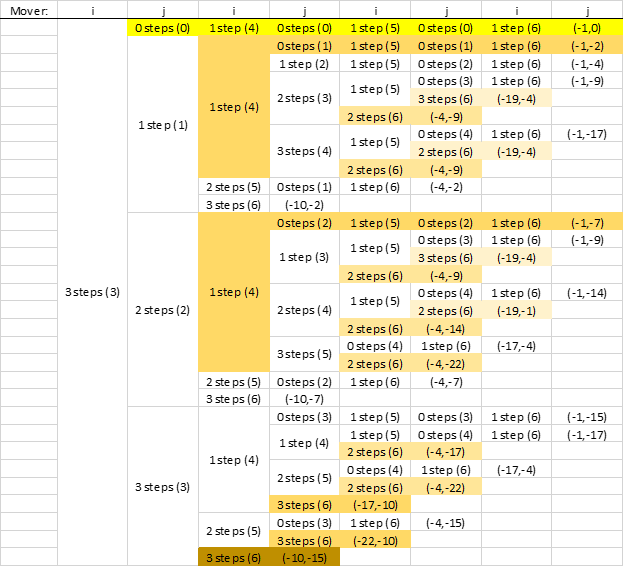
\includegraphics[scale=.5]{table4a.png}
		\end{center}
	
	\item 
	
	
\end{enumerate}

%%%________________________________________________________________%%%

\subsection*{Question 5}


%%%________________________________________________________________%%%

\subsection*{Question 5}

\begin{enumerate}[(a)]
	\item 
	
	
	\item 
	
	
	\item 
	
	
\end{enumerate}


%%%________________________________________________________________%%%


\end{document}




































